\chapter{Cocktail Party Introduction}

This thesis describes experimental research in fundamental physics, in particular I describe work on instrumentation, data analysis, and scientific interpretation for experiments aiming to study the nature of the first stars and galaxies, and how their formation affected the universe as a whole. This cocktail party introduction aims to introduce this research and its context to a non-technical audience. To introduce our immediate field of 21\,cm cosmology and the cosmic dawn, and its study with wide field radio interferometers, let us consider first why we are even studying this at all, and indeed what fundamental physics is in the first place. So many hear about this sort of research, and indeed its very incremental results, and simply ask \emph{Why?} I hope this gentle introduction begins to answer that question. Technically inclined readers should skip to Ch. 2.

\section[What is fundamental physics? \emph{So...you study string theory?}]{What is fundamental physics?\\ \emph{\large{So...you study string theory?}}}
%fundamental vs theoretical physics

Many people hear fundamental physics and think of theoretical physics like string theory. In fact, physics research might be fundamental, or it might be theoretical, or even both, or neither. Pop culture often glosses over the fact that the two terms are not synonymous, they are in fact distinct descriptors and refer to different aspects of the research. I find it useful to illustrate this distinction by classifying research on a 2D grid where the vertical axis goes from experimental to theoretical, and the horizontal one goes from fundamental to applied, as in Figure \ref{fig:typesofphysicsresearch}. 

I don't mean to classify research \emph{topics}, such as atoms or galaxies or superconductors, which often grow tentacles in all more than one quadrant, rather research \emph{types}, which are more related to the specific techniques employed. Experimental research typically involves building instruments and collecting and analyzing data to check theories, while theoretical research often involves proposing new theories or making predictions from pre-existing ones using analytic or numerical calculations. Fundamental research involves the basic laws of physics and nature of the universe from its fundamental building blocks, while applied research involves systems or models more immediately applicable society. 

\begin{figure}
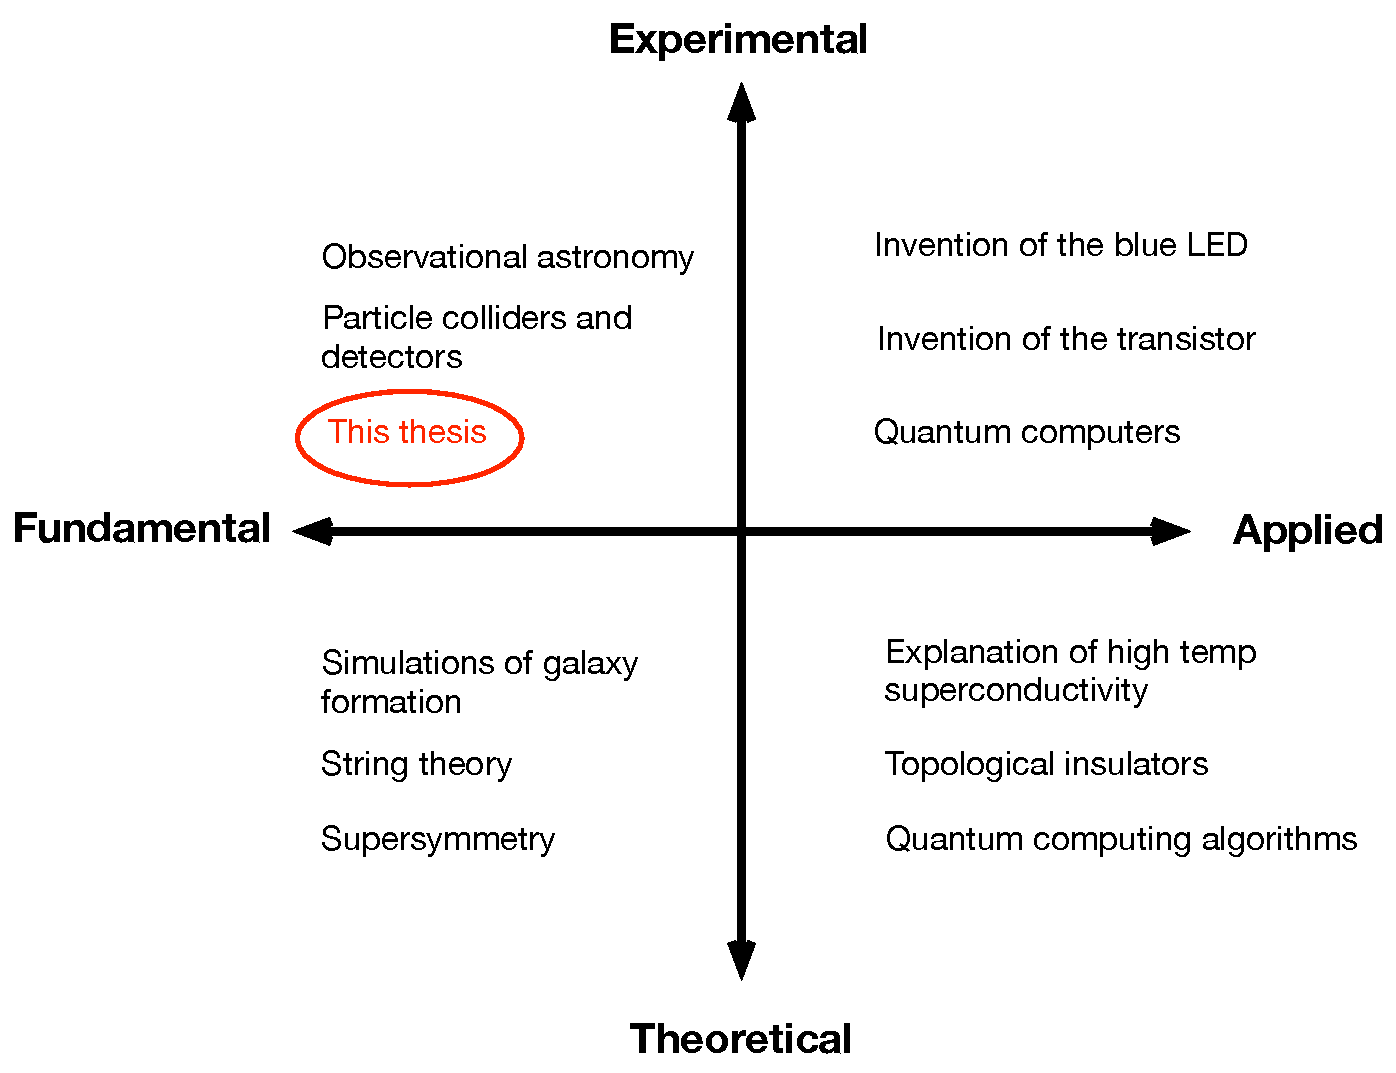
\includegraphics[width=6in]{cocktail_party_intro/types_of_physics_research.pdf}
\caption{A schematic diagram of physics research, from fundamental to applied, and experimental to theoretical, as well as several examples in each quadrant. Research topics often start in one quadrant and spread tentacles into others. Often, over time, fundamental research becomes more applied and theoretical research becomes more experimental, but sometimes the opposite happens, or neither. }
\label{fig:typesofphysicsresearch}
\end{figure}

To start to answer the \emph{Why?} of this thesis, let us consider the two fundamental quadrants. The fundamental--theoretical quadrant contains work like string theory and supersymmetry, and well as simulations designed to better elucidate the predictions of fundamental physics. This research often involves long calculations and heady math. Theorists often work in office complexes with endless supplies of white boards, and progress is made by thinking about a problem for a long time. Shoes aren't required, though many wear socks. Pencils are required, as well as the occasional computer to help evaluate the equations. To be sure, modern society would not exist without this quadrant. From Maxwell's electromagnetism to Einstein's relativity, what was originally fundamental theoretical became later became experimental and applied with the advent of radio, optical, and GPS technology. In other fields, such as quantum mechanics, fundamental theories and experiments developed in concert, but in all cases, the theoretical--fundamental understanding elucidated a crucial piece of the puzzle. 

Let's move on to the experimental--fundamental quadrant, which contains experimental work conducted to shed light on fundamental theories of nature. By fundamental I mean theories describing the building blocks of nature, or the fundamental properties of our universe. Sometimes the lines become blurry. Does chemistry belong here? Does biology? I would argue that because the understanding in these fields is largely empirical, and because they have yet to reach the point where a first principles approach is useful, these do not belong on our diagram of physics research. Astronomy is another difficult case, even as recently as a century ago astronomers, classification of galaxies into essentially arbitrary shape categories constituted a breakthrough. Over the twentieth century though, astronomy underwent a transformation into a field where practitioners observe astrophysical systems, test first principles-based theories or their behavior, and make quantitative predictions, to the point where many not refer to it as \emph{astrophysics}. Particle colliders are another example of research in this experimental--fundamental quadrant. 
 
Experimentalists build and use complex apparatuses to establish controlled conditions to test quantitative predictions of systems specifically sought out to study some fundamental property of nature. Many work in labs and shoes are nearly always required. We are lucky to have the generous support of institutions such as the Department of Energy, NASA, the National Science Foundation, as well as some private foundations to pursue this often expensive research which is almost always years, decades, or even centuries away from application.


\section[What is modern cosmology? \emph{Do you believe in the big bang?}]{What is modern cosmology?\\ \emph{\large{Do you believe in the big bang?}}}
%observational cosmology

The big bang is like biological evolution, the non-technical world makes a big fuss about it, but most scientists simply shake their heads and move on. Our understanding of biology and astronomy are so inextricably linked with these theories that there would practically be nothing left if we suddenly decided to reject them. A second point is that \textit{belief} not the most useful word here, or in science generally. To be sure, science requires at least a working belief that we live in a physical universe governed by mathematical laws, but if a scientific theory were backed up by so little data that it required \textit{belief} to be accepted, then it's unlikely to be very useful. There's an intermediate ground, of course, for theories in development or proposed before technology exists to test them, which no one would suggest discarding outright, but which aren't said to be ``accepted'' either. Rather, scientists say about string theory and supersymmetry, for instance, that the jury is still out.

In this section, I will discuss the modern field of cosmology and the evidence which puts the big bang squarely in the realm of fact. First, though, an important point about terminology. Many scientists and science popularizers play fast and loose with what the term `big bang' actually refers to. Does it refer to the predicted singularity 13.8 billion years ago when the whole observable universe fit on the head of a pin? Or both the singularity and its aftermath? Just its immediate aftermath, or the resulting expansion continuing into the present day? Or does it refer to the theory which predicts that that event? I suspect this ambiguity arises in part out of efforts to wow audiences at science lectures, and in part because the definition of the `big bang' is really beside the point in the technical literature. Experimentalists build instruments and study distant galaxies and theorists work to better understand the quantum field theory and general relativity. Editors don't make a big deal over the precise vocabulary used in paper introductions. Because of all this ambiguity, and because of the baggage the term `big bang' carries among the public, I prefer not to use it at all. Let's just discuss what we know.

I \textit{could} just describe our modern picture of the Galaxy, the universe and cosmology, but I fear it would be all to easy to simply dismiss it as a philosophy just like any other. So the purpose of this cocktail party introduction, I'll take a more historical approach and describe the main breakthroughs over the past century that have made cosmology the precision science that it is today. 

Our story begins in the early 1920s, by which time a number of poorly understood \textit{spiral nebulae}, fuzzy spiral blobs, had been observed in the night sky. There were essentially two possibilities. On the one hand, perhaps they were cloud of gas in the far reaches of our own galaxy; on the other, perhaps they were galaxies like our own but just farther away than object every seen before. The implications were enormous. Is there our galaxy all there is, or is it part of a space even more vast with countless others? Things came to a head in the famous Great Debate between astronomers Harlow Shapley and Heber Curtis at the Smithsonian in 1920 \citep{greatdebate}. The debate itself was mostly a stunt, scientific disputes aren't settled by debate but by better data. There were measurements that supported both points of view, but none of the data were extremely convincing. The dispute wasn't settled until Edwin Hubble, using the new 100\,in Palomar telescope on Mount Wilson, made the first measurements of the distances to these spiral nebulae, and demonstrated they were way outside our galaxy \citep{hubble26}. Hubble sought and monitored a type of pulsating stars in these nebulae called Cepheid variables, which are known to pulsate with a period proportional to their intrinsic brightness. Then by comparing their \textit{apparent} brightness, more distant objects generally appearing dimmer, their distances could be obtained. Many of the spiral nebulae were millions of light-years away, while our galaxy was known to be only about 50,000 light-years from side to side. The debate was settled, the universe was much larger than we had known.

For his next trick, Hubble turned his attention to even more distant galaxies, and the results were just as shocking. With only a few exceptions all appeared to be flying away from us at staggering velocities, hundreds or thousands of kilometers per second. Fast enough to travel around the earth in less than a minute. Moreover more distant galaxies were flying away from us faster, linearly faster. Exactly what you'd expect for a uniform expansion of space-time itself. It was as if a balloon with dots on it was being inflated; no matter which dot you're sitting on, all others are moving away from you at a rate proportional to their distance. I have reproduced Hubble's original data in Fig. \ref{fig:hubbleslaw}, which shows that the recession velocities a galaxy rises linearly with its distance. This relationship is known as Hubble's law, and the coefficient of proportionality, in units of velocity per distance, is knowns as the Hubble constant. Modern measurements place this value at roughly 70\,km/s/Mpc \citep{reiss16,planck16}, where 1\,Mpc = 1,000,000 parsecs. 

\begin{figure}
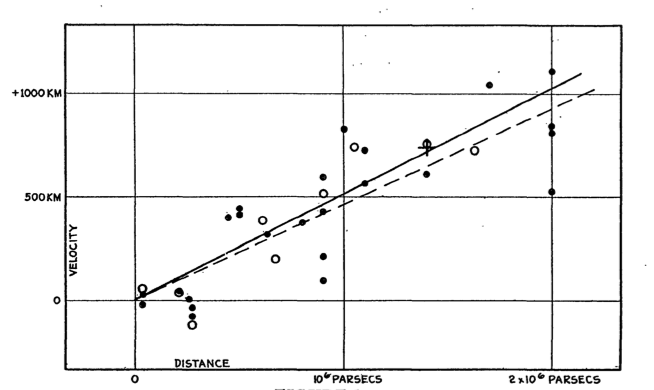
\includegraphics[width=6in]{cocktail_party_intro/hubble_diagram.png}
\caption{Hubble's measurements showed that galaxies in all directions are moving away from us at a speed linearly proportional to their distances. Here is his actual figure, reproduced from \citet{hubble29}, showing recession velocities of nearby galaxies in km/s (on the vertical axis) as a function of their distance from the Milky Way in parsecs (on the horizontal axis). Note 1 parsec is 3.26 light-years.}
\label{fig:hubbleslaw}
\end{figure}

How can the universe itself be expanding? What does that even mean? Einstein had applied the field equations of General Relativity to the universe as a whole and found that static solutions are impossible, which suggested to him that his equations were not completely correct. He found that a single constant added to the central field equation of the theory was sufficient to ensure a static solution, a \textit{cosmological constant} \citep{einstein17}. After hearing of Hubble's results, though, Einstein famously abandoned that addition, calling it his ``greatest mistake.'' It wasn't so much a \textit{mistake} per se, given that there wasn't any data at the time to test his prediction, more a missed opportunity. He could, after all, have gambled and \textit{predicted} the expansion of the Universe, and perhaps won a second Nobel prize for it.

Despite this early progress, cosmology was a research backwater for decades and for a time fell out of all memory, until the most unlikely creature of all, an engineer, made a breakthrough. In the course of developing ultra sensitive radio receivers at Bell Labs, Messrs. Anro Penzias and Robert Wilson were working with a horn antenna which seemed to pick up a very faint noise which they couldn't explain. 

Radio astronomers ofter quantify the power of radio emission by the equivalent temperature of a blackbody emitting the same amount of power. Let us build some intuition here, for a moment. Any object at a temperature $T$ emits electromagnetic radiation, the hotter it is, the higher frequency of the radiation. Objects at room temperature emit predominantly in the infrared band, while objects at a few thousand degrees, like the sun, emit in the optical band. At the other end of the spectrum, radio waves are emitted by very cold objects. Note of course that we are only talking about the  electromagnetic waves emitted by the random jostling around of atoms. By running currents through a wire, substantially more powerful radio waves may be produced which are not random at all, and are useful for transmitting Lady Gaga lyrics, among other things.

The background radiation detected by Penzias and Wilson was equivalent to that emitted by a very cold object, within a few degrees of absolute zero, 3 kelvin to be precise \citep{penzias65}. Moreover, it was the exact same brightness in any direction they looked away from our galaxy. Their discovery set off a flashbang in the cosmology community. Based on calculations of how nuclear fusion and fission calculations in a hot, dense early universe could account for the abundances of various stable and radioactive chemical elements, Ralph Alpher and Robert Herman calculated that the ambient temperature of empty space today to be roughly 5 kelvin \citep{alpher48,alpherherman,gamow48}.  The exact temperature was somewhat uncertain, and later estimates ranged from a few kelvin to tens of kelvin, but \citep{dicke65} immediately recognized that the observed 3 kelvin radiation was cosmic in origin, corresponding exactly to the aftermath of that hot, dense early state, what had been mocked as the `the big bang' by astronomers who opposed the theory. But much as it's a losing battle to keep non-scientists from referring the Higgs boson as `the God particle', the name `big bang' is not going anywhere soon. 

Two additional discoveries made in the early 1990s confirmed these results and set the stage for the more precise field of 21\,cm cosmology and the cosmic dawn that we address in this thesis. Both came from a satellite-born experiment named the Cosmic Background Explorer (COBE) designed to better study the cosmic microwave background discovered by Penzias and Wilson. The first key result was a precise measurement of its frequency spectrum. Man-made radiation or or experimental noise is rarely or never exactly thermal, that is, due only to random motions of atoms and electrons, and thus an exactly thermal spectrum is special. Radiation emitted by stars and galaxies ofter looks somewhat thermal, but atoms and dust inevitable emit or absorb some of it at different frequencies, always resulting in an imperfect frequency spectrum. In fact, the only known source of such a perfect thermal spectrum is the hot, dense early universe before galaxies had formed and everything was a sort of primordial soup, or more precisely, a purée. All scientific opposition to the hot, dense early universe model, ie, the `big bang' picture, evaporated after the publication of this spectrum, reproduced in Fig. \ref{fig:cobecmbspectrum}, published in \citep{cobespectrum,cobespectrum2}.

\begin{figure}
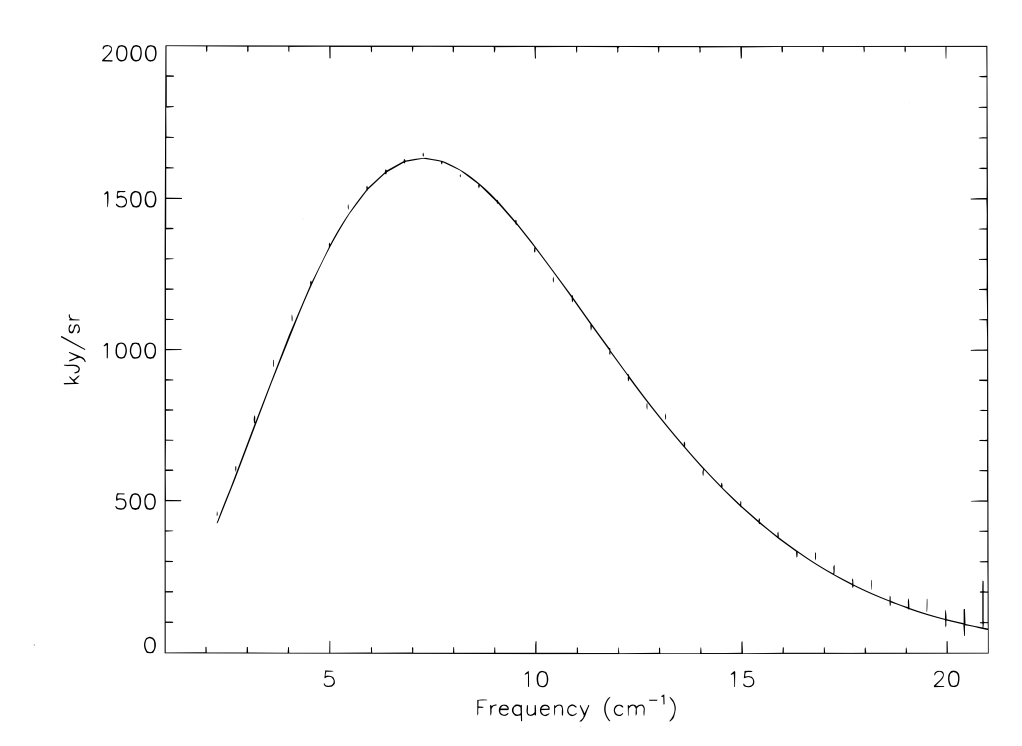
\includegraphics[width=6in]{cocktail_party_intro/cobe_cmb_spectrum.png}
\caption{CMB spectrum}
\label{fig:cobecmbspectrum}
\end{figure}


The second discovery was the icing on the cake. On top of clear evidence of the exotic hot, dense, homogenous early universe, COBE saw hints of how the modern \textit{clumpy} universe emerged. To the imprecise radio antenna of Penzias and Wilson, the cosmic microwave background appeared just as bright in every direction they looked. But the more sensitive COBE distinguished two interesting patterns. First, after subtracting the sky-averaged intensity corresponding to the 3 kelvin radiation, they observed a \textit{dipole} pattern in the sky. That is, the sky was uniformly brighter in one direction and fainter in the other, which was interpreted as the doppler shift of the cosmic microwave background due to the motion of our galaxy relative to other galaxies. It's as if our dot on the balloon is actually moving slowly across the balloon surface while the balloon is expanding, so dots on one side don't seem to be receeding as quickly, while those on the other appear to be receeding faster than they otherwise would. This \textit{anisotropy} of the cosmic microwave background shows us the slightly \textit{in}homogenieties in the nearly smooth early universe. 

\begin{figure}
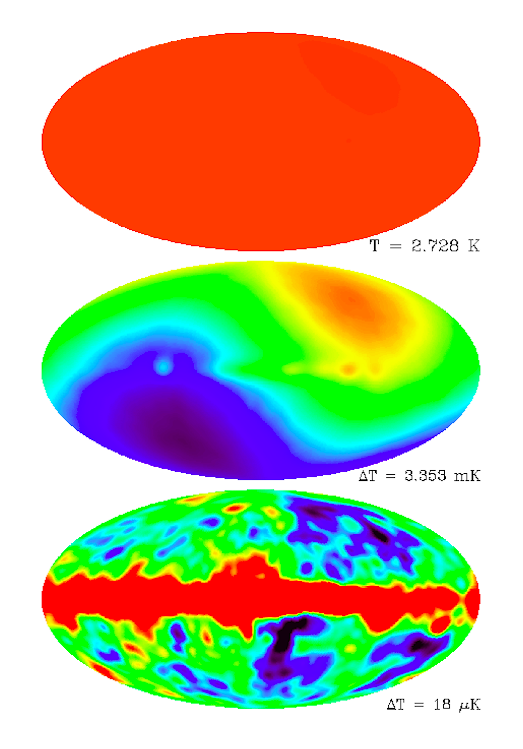
\includegraphics[width=6in]{cocktail_party_intro/cobe_cmb_anisotropy.png}
\caption{CMB anisotropy}
\label{fig:cobecmbanisotropy}
\end{figure}

Over time, we predict, but have yet to directly observe, that the denser regions slowly drew in more matter and collapsed due to gravitational attraction, eventually forming many galaxies. More recent CMB surveys by the WMAP \citep{wmap9year} and Planck \citep{planck15} satellites have confirmed and extended these results with exquisite precision, and truly made the past two decades the golden age of cosmology.


Lastly, I would be remiss if I didn't mention the most shocking discovery in cosmology over the past decades: the acceleration of the expansion of the universe. It does not directly relate to the work in this thesis, but it ties back to a thread discussed earlier. In 1997 and 1998, two groups attempting to reproduce, refine, and extend Hubble's original measurements (Fig. \ref{fig:hubbleslaw} to more distant galaxies, observed that galaxies a thousand times more distant that Hubble's appeared 
% 0.5 magnitudes is 10^(-0.5/2.5) = ~0.6
only half as bright as they should \citep{perlmutter97,riess08}. An obvious possibility is obscuration by dust, but both groups went to great lengths to demonstrate this was not the case. Dust absorbs preferentially red light, drastically altering the spectrum, but the spectra of these galaxies appeared normal. They were just fainter than their other properties suggested they should be. The consensus conclusion is that not only is the universe is expanding, but it is accelerating, due to exactly a term in Einstein's field equation like the cosmological constant he artificially added. But this time with living proof.

\section[What is the cosmic dawn? \emph{How did stars and galaxies form?}]{What is the cosmic dawn?\\ \emph{\large{How did stars and galaxies form?}}}
 
brief summary of the timeline of the universe, building on what we've learned in the previous section
nucleosynthesis, dark ages, cosmic dawn / reionization, modern universe / acceleration
highlight that CMB and dark galaxy surveys have closed in on the cosmic dawn, but it is the last major piece of the puzzle

why was the cosmic dawn an important and interesting epoch
pop III stars and reionization

pop III stars: what we know and don't know

reionization: what we know and don't know

the major problem: how do we study the universe before there were stars?

\section[21\,cm cosmology. \emph{How can we see into the darkness?}]{21\,cm cosmology\\ \emph{\large{How can we see into the darkness?}}}

solution to seeing into the epoch before stars: studying the faint radio emission from hydrogen gas
note: universe is 75\% hydrogen!
study evolution over time and space ==> tomography

hydrogen line and hyperfine transition
used in galactic astronomy to measure galactic rotation curve
intuitive physics of the hyperfine transition
1.4GHz line

redshifts to low frequency band
renaissance of low freq (100s of MHz) radio astronomy
how do interferometers work?
much cheaper than giant dishes, not possible with computing


